\begin{frame}
\frametitle{Paraméter választás\uncover<2>{: fokszám}}

\begin{columns}
\begin{column}{0.5\textwidth}
\begin{footnotesize}
\begin{itemize}
\item Csúcsok száma: $n$ (pl. $1000$)
\item Kizárható vendégek száma: $k$ (pl. $10$)
\uncover<2>{\item\textcolor{red}{Csúcsok fokszáma: $1\leq{}d(v)\leq{}k$}}
\end{itemize}
\emptyline
Mit tehetünk a következő csúcsokkal?
\begin{itemize}
\item A: $0$ fokszámú csúcs\\
\uncover<2>{\footnotesize{\textcolor{red}{$\rightarrow$ Beengedhető, nem ronthatja el}}}
\item B: $k+1\leq$ fokszámú csúcs\\
\uncover<2>{\footnotesize{\textcolor{red}{$\rightarrow$ Mindenképp ki kell zárni}}}\\
\uncover<2>{\footnotesize{\textcolor{red}{$\rightarrow$ k-t csökkenteni 1-el}}}
\end{itemize}
\end{footnotesize}
\end{column}

\begin{column}{0.5\textwidth}
\begin{center}
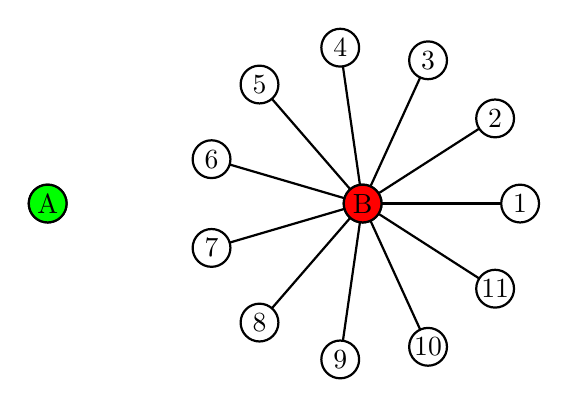
\begin{tikzpicture}[scale=2]
\coordinate (N1)  at (3.00000,1.00000);
\coordinate (N2)  at (2.84125,1.54064);
\coordinate (N3)  at (2.41542,1.90963);
\coordinate (N4)  at (1.85769,1.98982);
\coordinate (N5)  at (1.34514,1.75575);
\coordinate (N6)  at (1.04051,1.28173);
\coordinate (N7)  at (1.04051,0.71827);
\coordinate (N8)  at (1.34514,0.24425);
\coordinate (N9)  at (1.85769,0.01018);
\coordinate (N10) at (2.41542,0.09037);
\coordinate (N11) at (2.84125,0.45936);
\coordinate (A)   at (0.00000,1.00000);
\coordinate (B)   at (2.00000,1.00000);
\draw[thick] (B) -- (N1);
\draw[thick] (B) -- (N2);
\draw[thick] (B) -- (N3);
\draw[thick] (B) -- (N4);
\draw[thick] (B) -- (N5);
\draw[thick] (B) -- (N6);
\draw[thick] (B) -- (N7);
\draw[thick] (B) -- (N8);
\draw[thick] (B) -- (N9);
\draw[thick] (B) -- (N10);
\draw[thick] (B) -- (N11);
\draw[thick, fill=white] (N1)  circle (0.12) node{1};
\draw[thick, fill=white] (N2)  circle (0.12) node{2};
\draw[thick, fill=white] (N3)  circle (0.12) node{3};
\draw[thick, fill=white] (N4)  circle (0.12) node{4};
\draw[thick, fill=white] (N5)  circle (0.12) node{5};
\draw[thick, fill=white] (N6)  circle (0.12) node{6};
\draw[thick, fill=white] (N7)  circle (0.12) node{7};
\draw[thick, fill=white] (N8)  circle (0.12) node{8};
\draw[thick, fill=white] (N9)  circle (0.12) node{9};
\draw[thick, fill=white] (N10) circle (0.12) node{10};
\draw[thick, fill=white] (N11) circle (0.12) node{11};
\uncover<1>{\draw[thick, fill=white] (A)   circle (0.12) node {A};}
\uncover<2>{\draw[thick, fill=green] (A)   circle (0.12) node {A};}
\uncover<1>{\draw[thick, fill=white] (B)   circle (0.12) node {B};}
\uncover<2>{\draw[thick, fill=red]   (B)   circle (0.12) node {B};}
\end{tikzpicture}
\end{center}
\end{column}
\end{columns}

\end{frame}

